\begin{figure}
  \centering
  \begin{subfigure}[b]{0.5\textwidth}
    \begin{adjustbox}{minipage=\textwidth, scale=0.5}
      \usetikzlibrary{calc,angles, positioning}
      \tikzstyle{array_element}=[rectangle,
        minimum height=2cm,
        minimum width=2cm,
        minimum size=3cm,
        draw=black,
        rounded corners=2.5, ]

      \definecolor{LightColor}{rgb}{1.0,0.951,0.905}
      \definecolor{tile2}{HTML}{B5EDCD}
      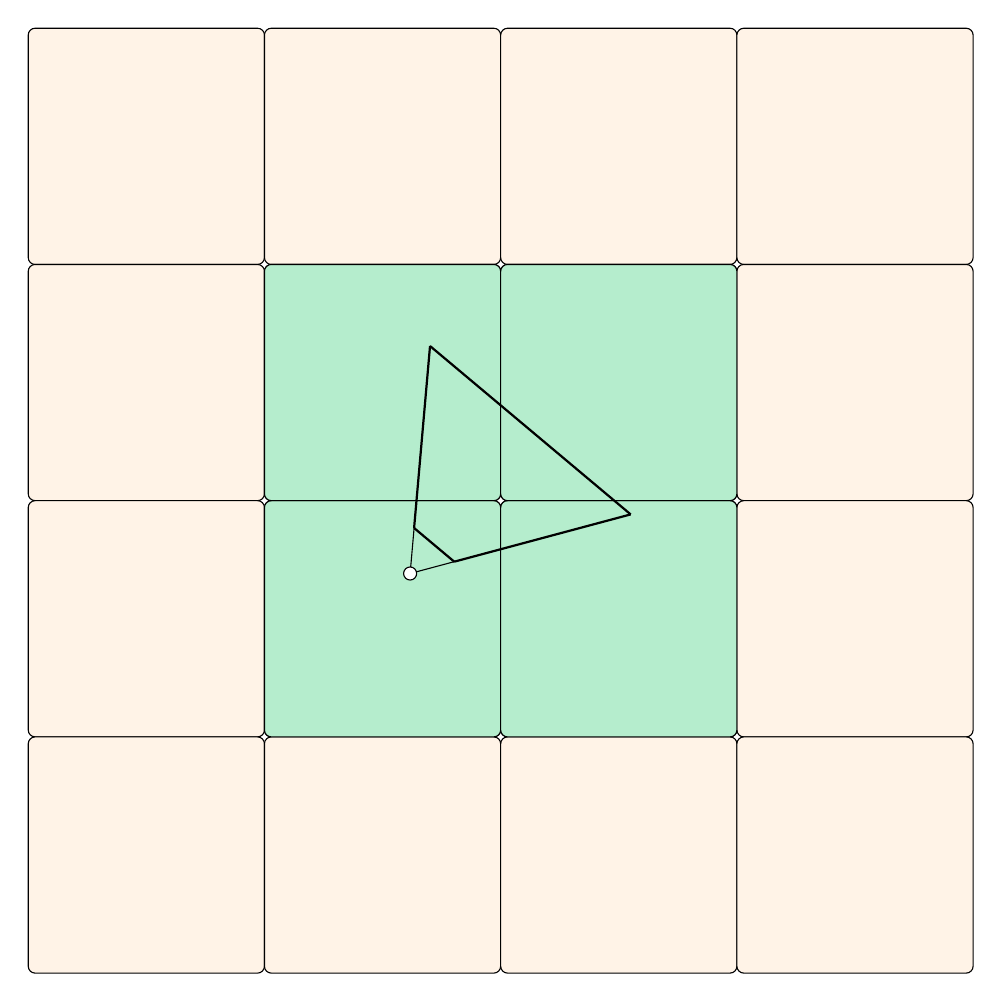
\begin{tikzpicture}
    \foreach \la in {0,...,3} {
        \foreach \lb in {0,...,3} {
            \node at (3cm * \la, -3cm * \lb) (H\la\lb) [array_element, fill=LightColor] {};
        }
    }
\node at (3cm * 1, -3cm *2) (H) [array_element, fill=tile2] {};
\node at (3cm * 1, -3cm *1) (H) [array_element, fill=tile2] {};
\node at (3cm * 2, -3cm *2) (H) [array_element, fill=tile2] {};
\node at (3cm * 2, -3cm *1) (H) [array_element, fill=tile2] {};

    \coordinate [] (origin) at (3.35cm, -5.425cm);
    \coordinate [] (v) at (3.35cm + 2.9cm, -5.425cm);
    \node at ((3.35cm + 0.2 * 2.801cm, -5.425cm + 0.2 * 0.7506cm) [] (val11) {};
    \node at ((3.35cm + 0.2 * 0.2528cm, -5.425cm + 0.2 * 2.889cm) [] (val12) {};

    \node at ((3.35cm + 2.801cm, -5.425cm + 0.7506cm) [] (val21) {};
    \node at ((3.35cm + 0.2528cm, -5.425cm + 2.889cm) [] (val22) {};
    
    \draw[-, thick] (val11.center) -- (val12.center);
    \draw[-, thick] (val21.center) -- (val22.center);
    \draw[-, thick] (val12.center) -- (val22.center);
    \draw[-, thick] (val11.center) -- (val21.center);
    \draw[-] (val11.center) -- (origin.center);
    \draw[-] (val12.center) -- (origin.center);
    \node at (origin) (origin-node) [circle, draw, scale=0.5, fill=white] {};  

\end{tikzpicture}
    \end{adjustbox}
  \caption{Opdeling met behulp van $2^3$ stukken.}
  \label{fig:vo-subsets:2}
  \end{subfigure}%
  \begin{subfigure}[b]{0.5\textwidth}
    \begin{adjustbox}{minipage=\textwidth, scale=0.5}
      \usetikzlibrary{calc, angles, positioning}
  \tikzstyle{array_element}=[rectangle,
                             minimum height=2cm, 
                             minimum width=2cm, 
                             minimum size=3cm,
                             draw=black,
                             rounded corners=2.5, ]
                             
                             \definecolor{LightColor}{rgb}{1.0,0.951,0.905}
\definecolor{tile2}{HTML}{B5EDCD}
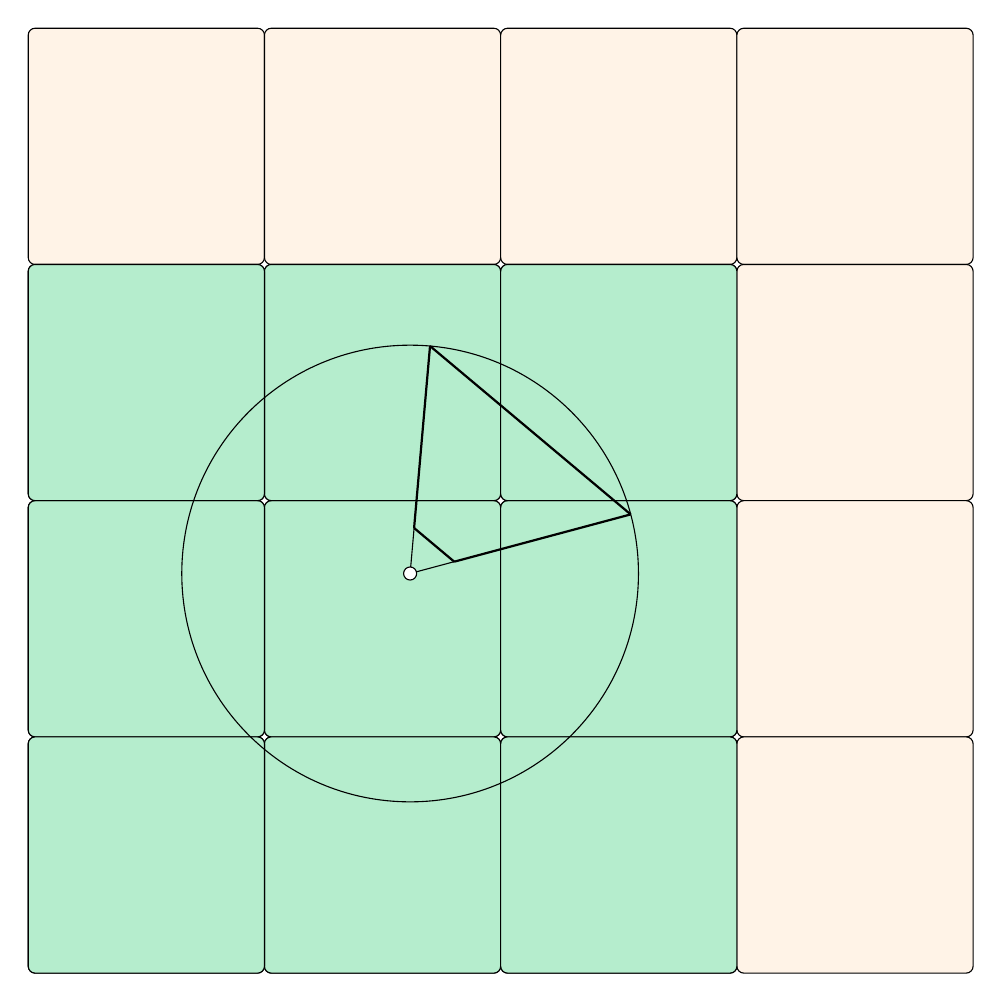
\begin{tikzpicture}
    \foreach \la in {0,...,3} {
        \foreach \lb in {0,...,3} {
            \node at (3cm * \la, -3cm * \lb) (H\la\lb) [array_element, fill=LightColor] {};
        }
    }
\node at (3cm * 1, -3cm *2) (H) [array_element, fill=tile2] {};
\node at (3cm * 1, -3cm *1) (H) [array_element, fill=tile2] {};
\node at (3cm * 1, -3cm *3) (H) [array_element, fill=tile2] {};

\node at (3cm * 2, -3cm *2) (H) [array_element, fill=tile2] {};
\node at (3cm * 2, -3cm *1) (H) [array_element, fill=tile2] {};
\node at (3cm * 2, -3cm *3) (H) [array_element, fill=tile2] {};

\node at (3cm * 0, -3cm *2) (H) [array_element, fill=tile2] {};
\node at (3cm * 0, -3cm *1) (H) [array_element, fill=tile2] {};
\node at (3cm * 0, -3cm *3) (H) [array_element, fill=tile2] {};

    \coordinate [] (origin) at (3.35cm, -5.425cm);
    \coordinate [] (v) at (3.35cm + 2.9cm, -5.425cm);
    \node at ((3.35cm + 0.2 * 2.801cm, -5.425cm + 0.2 * 0.7506cm) [] (val11) {};
    \node at ((3.35cm + 0.2 * 0.2528cm, -5.425cm + 0.2 * 2.889cm) [] (val12) {};

    \node at ((3.35cm + 2.801cm, -5.425cm + 0.7506cm) [] (val21) {};
    \node at ((3.35cm + 0.2528cm, -5.425cm + 2.889cm) [] (val22) {};
    
    \draw[-, thick] (val11.center) -- (val12.center);
    \draw[-, thick] (val21.center) -- (val22.center);
    \draw[-, thick] (val12.center) -- (val22.center);
    \draw[-, thick] (val11.center) -- (val21.center);
    \draw[-] (val11.center) -- (origin.center);
    \draw[-] (val12.center) -- (origin.center);
    \node at (origin) (origin-node) [circle, draw, scale=0.5, fill=white] {};
    \node at (origin) (origin-node) [circle, draw, minimum size = 5.8cm] {};  

\end{tikzpicture}
    \end{adjustbox}
  \caption{Opdeling met behulp van $3^3$ stukken.}
  \label{fig:vo-subsets:3}
  \end{subfigure}%
  \caption{Opdeling van de sc\`eneruimte.}
  \label{fig:vo-subsets}
\end{figure}
